\documentclass[english,11pt]{article}
\usepackage[T1]{fontenc}
\usepackage[latin9]{inputenc}
\usepackage{amsmath}
\usepackage{amsthm, amsfonts}
\usepackage{fullpage}
\usepackage[margin=1in]{geometry}
\usepackage{amssymb}
\usepackage{graphicx}
\usepackage{subcaption}
\usepackage{braket}
\usepackage{enumitem}
\usepackage{thmtools,thm-restate}
\usepackage{xcolor}
\usepackage{tikz}
\usetikzlibrary{quantikz}
\usepackage[bookmarks=false]{hyperref}
\definecolor{darkgreen}{rgb}{0,0.5,0}
\hypersetup{linktocpage=true,colorlinks=true,citecolor=red,linkcolor=darkgreen}

\usepackage[ruled,vlined,linesnumbered]{algorithm2e}

\newtheorem{theorem}{Theorem}[section]
\newtheorem{claim}[theorem]{Claim}
\newtheorem{proposition}[theorem]{Proposition}
\newtheorem{lemma}[theorem]{Lemma}
\newtheorem{corollary}[theorem]{Corollary}
\newtheorem{conjecture}[theorem]{Conjecture}
\newtheorem{remark}[theorem]{Remark}
\newtheorem{definition}[theorem]{Definition}
\makeatletter

\newcommand{\expref}[2]{{\texorpdfstring{\hyperref[#2]{#1~\ref{#2}}}{#1~\ref{#2}}}} 
\newcommand{\secref}[1]{\expref{Section}{#1}}
\newcommand{\thmref}[1]{\expref{Theorem}{#1}}
\newcommand{\clmref}[1]{\expref{Claim}{#1}}
\newcommand{\tref}[1]{\expref{Theorem}{#1}}
\newcommand{\appref}[1]{\expref{Appendix}{#1}}
\newcommand{\lref}[1]{\expref{Lemma}{#1}}
\newcommand{\corref}[1]{\expref{Corollary}{#1}}
\newcommand{\conjref}[1]{\expref{Conjecture}{#1}}
\newcommand{\pref}[1]{\expref{Proposition}{#1}}
\newcommand{\figref}[1]{\expref{Figure}{#1}}

\captionsetup[subfigure]{subrefformat=simple,labelformat=simple,listformat=subsimple}
\renewcommand\thesubfigure{(\alph{subfigure})}


%%%%%%%%%%%%%%%%%%%%%%%%%%%%%% Textclass specific LaTeX commands.
\theoremstyle{plain}
\newtheorem{thm}{\protect\theoremname}
\theoremstyle{plain}
\newtheorem{lem}[thm]{\protect\lemmaname}
\theoremstyle{remark}
\newtheorem{rem}[thm]{\protect\remarkname}

%%%%%%%%%%%%%%%%%%%%%%%%%%%%%% User specified LaTeX commands.
\usepackage{algorithmic}

\makeatother
\renewcommand{\deg}{\mathrm{deg}}
\renewcommand{\inf}{\mathrm{Inf}}
\newcommand{\Inf}{\mathrm{Inf}}
\newcommand{\maxinf}{\mathrm{MaxInf}}
\newcommand{\bs}{\mathrm{bs}}
\newcommand{\D}{\mathrm{D}}
\newcommand{\poly}{\mathrm{poly}}
\newcommand{\ui}{{\boldsymbol{i}}}
\newcommand{\eps}{\epsilon}
\usepackage{babel}
\providecommand{\lemmaname}{Lemma}
\providecommand{\remarkname}{Remark}
\providecommand{\theoremname}{Theorem}
\usepackage{color}
\newcommand{\ba}{{{a}}}
\newcommand{\R}{{\mathbb R}}
\newcommand{\N}{\mathbb{N}}
\newcommand{\C}{\mathbb{C}}
\newcommand{\pmone}{\{\pm 1\}}
\newcommand{\cbnorm}[1]{\|#1\|_{\mathrm{cb}}}
\newcommand{\Mnote}[1]{{\color{orange} {\bf Makrand: } #1}}
\newcommand{\Rnote}[1]{{\color{blue} {\bf RdW: } #1}}
\newcommand{\Nnote}[1]{{\color{red} {\bf Nikhil: } #1}}
\newcommand{\hl}[1]{\textcolor{blue}{#1}}
\newcommand{\E}{\mathbb{E}}
\newcommand{\Ef}{\E f}
\newcommand{\BZ}{\mathbf{0}}
\newcommand{\I}{\mathbb{I}}
\newcommand{\Diag}{\mathrm{Diag}}
\newcommand{\beq}{\begin{equation}}
\newcommand{\eeq}{\end{equation}}
\newcommand{\hT}{\widehat{T}}
\newcommand{\Var}{\mathrm{Var}}
\newcommand{\CP}{\mathcal{P}}
\newcommand{\NC}{\mathcal{NC}}
\newcommand{\bi}{{\boldsymbol{i}}}
\newcommand{\bj}{{\boldsymbol{j}}}
\newcommand{\comment}[1]{{}}
\newcommand{\BU}{\boldsymbol{U}}
\newcommand{\U}{\boldsymbol{U}}
\newcommand{\BA}{\mathbf{A}}
\newcommand{\BM}{\mathbf{M}}
\newcommand{\x}{\boldsymbol{x}}

\newcommand{\CA}{\mathcal A}
\newcommand{\bone}{\boldsymbol{1}}
\newcommand{\bzero}{\boldsymbol{0}}
%\newcommand{\C}{\mathbb C}
\newcommand{\tr}{\mathrm{tr}}
\newcommand{\BR}{\R}
\newcommand{\BN}{\N}
\newcommand{\CB}{\mathcal{B}}
\newcommand{\sM}{\mathsf{M}}
\newcommand{\sA}{\mathsf{A}}
\newcommand{\ind}{\mathbf{1}}
\newcommand{\op}{\mathrm{op}}
\newcommand{\BE}{\E}
\newcommand{\fhat}{\widehat{f}}
\newcommand{\del}{\partial}
\newcommand{\fix}{\mathsf{fix}}
\newcommand{\free}{\mathsf{free}}
\newcommand{\cb}{\mathrm{cb}}
\newcommand{\hf}{\widehat{f}}
\newcommand{\bb}{\boldsymbol{b}}
\renewcommand{\phi}{\varphi}
\date{} 

\begin{document}

\title{Influence in Completely Bounded Block-multilinear Forms and Classical Simulation of Quantum Algorithms}
\author{ Nikhil Bansal\thanks{\texttt{bansaln@umich.edu}. Supported in part by the NWO VICI grant 639.023.812.}\\ \small University of Michigan \and
 Makrand Sinha\thanks{\texttt{makrand@berkeley.edu}. Supported by a Simons-Berkeley postdoctoral fellowship.}\\ \small Simons Institute and UC Berkeley \and 
 Ronald de Wolf\thanks{\texttt{rdewolf@cwi.nl}. Partially supported by the Dutch Research Council (NWO/OCW), as part of the Quantum Software Consortium programme (project number 024.003.037), and through QuantERA ERA-NET Cofund project QuantAlgo (680-91-034).}\\ \small{QuSoft, CWI and U.\ of Amsterdam}
}

\maketitle
\begin{abstract}
The Aaronson-Ambainis conjecture (Theory of Computing '14) says that every low-degree bounded polynomial on the Boolean hypercube has an influential variable. This conjecture, if true, would imply that the acceptance probability of every $d$-query quantum algorithm can be well-approximated almost everywhere (i.e., on almost all inputs) by a $\poly(d)$-query classical algorithm.
We prove a special case of the conjecture: in every completely bounded  degree-$d$ block-multilinear form with constant variance, there always exists a variable with influence at least $1/\poly(d)$. In a certain sense, such polynomials characterize the acceptance probability of quantum query algorithms, as shown by Arunachalam, Bri\"et and Palazuelos (SICOMP '19). As a corollary we obtain efficient classical almost-everywhere simulation for a particular class of quantum algorithms that includes for instance $k$-fold Forrelation.
Our main technical result relies on connections to free probability theory.
\end{abstract}


\thispagestyle{empty}
\clearpage
\newpage
\setcounter{page}{1}

\allowdisplaybreaks

Reinforcement learning has achieved great success in areas such as Game-playing \citep{silver2018general,vinyals2019grandmaster}, robotics \cite{kober2013reinforcement}, large language models \citep{ouyang2022training}, etc.
However, due to safety concerns or physical limitations, in some real-world reinforcement learning problems, we must consider additional constraints that may influence the optimal policy and the learning process \citep{garcia2015comprehensive}.
% For example, a robotic arm must not take actions that may cause harm to itself or the environments.
A standard framework to handle such cases is the constrained Markov Decision Process (CMDP) \citep{altman1999constrained}.
Within the CMDP framework, the agent has to maximize
the expected cumulative reward while
obeying a finite number of constraints, which are usually in the form of expected cumulative cost criteria.

However, we are sometimes concerned with the problem with a continuum of constraints.
For example,
the constraints we meet might be time-evolving or subject to uncertain parameters, which
cannot be formulated as an ordinary CMDP
(see Examples \ref{Example_Time_Evolving} and  \ref{Example_Uncertain}).
In this paper we would study a generalized CMDP  
to address the above problem.  Because the constraints are not only infinite-number but also lie
in a continuous set,
the generalization is not trivial. Fortunately, we find that we can borrow the idea behind semi-infinite programming (SIP) \citep{remez1934determination, hettich1993semi} to deal with the semi-infinite constraints.
Accordingly, we propose \emph{semi-infinitely constrained Markov decision processes} (SICMDPs)
as a novel complement to the ordinary CMDP framework.
%More specifically,  an SICMDP model %, we consider 
%contains a continuum of constraints whereas an ordinary CMDP contains a finite number of constraints. 

%This generalization is natural but not trivial. However, we can brows the idea  
%The idea is quite natural and can be backtracked
%to the practice of extending linear programming to linear semi-infinite programming (LSIP) %\cite{remez1934determination, GobernaLSIO1998}.
%In addition, 
%As a complementary approach to the ordinary CMDP framework, 
%SICMDP can be used to model these problems  which cannot be described by a finite number of constraints
%that are not covered by .
%For example,
%the restrictions we consider can be time-evolving or subject to uncertain parameters
%, thus
%cannot be described by a finite number of constraints but a continuum of constraints 
%(see Examples \ref{Example_Time_Evolving} and  \ref{Example_Uncertain}).

We also present two reinforcement learning algorithms to solve SICMDPs called SI-CRL and SI-CPO, respectively.
SI-CRL is a model-based reinforcement learning algorithm designed for tabular cases, and SI-CPO is a policy optimization algorithm for non-tabular cases.
% and analyze its performance both theoretically and empirically.
The main challenge is that we need to deal with a continuum of constraints, thus reinforcement learning algorithms for ordinary CMDPs do not work anymore.
In SI-CRL, we tackle this difficulty by first transforming the reinforcement learning problem to an equivalent LSIP problem, which can then be solved using methods in the LSIP literature like the dual exchange methods \citep{Hu1990,reemtsen1998numerical}.
In SI-CPO, we resort to the idea of cooperative stochastic approximation developed in \cite{lan2020algorithms, wei2020comirror}.
As far as we know, we are the first to introduce tools from semi-infinitely programming (SIP) into the reinforcement learning community for solving constrained reinforcement learning problems.

% To the best of our knowledge, we are the first to apply tools from semi-infinitely programming (SIP) to solve reinforcement learning problems.
Furthermore, we give theoretical analysis for both SI-CRL and SI-CPO.
We decompose the error of SI-CRL into two parts: the statistical error from approximating the true SICMDP with an offline dataset and the optimization error due to the fact that the solution of the LSIP problem obtained by the dual exchange method is inexact.
On the optimization side, we show that the iteration complexity of SI-CRL is $O\left(\left\{\mathrm{diam}(Y)L\sqrt{|\gS|^2|\gA|m}/\left[(1-\gamma)\epsilon\right]\right\}^m\right)$.
On the statistical side, we show that the sample complexity of SI-CRL is $\widetilde O\left(\frac{|S|^2|A|^2}{\epsilon^2(1-\gamma)^3}\right)$ if the offline dataset is generated by a generative model, and $\widetilde O\left(\frac{|S||A|}{\nu_{\min} \epsilon^2(1-\gamma)^3}\right)$ if the dataset is generated by a probability measure $\nu$ as considered in \cite{chen2019information}.
Here $\widetilde O$ means that all logarithm terms are discarded.
For SI-CPO, things become a little more complicated because other than the statistical error and the optimization error, we also need to consider the function approximation error, which comes from imperfect policy parametrizations.
It is shown if the function approximation error can be controlled to $O(\epsilon)$ order, the iteration complexity of SI-CPO is $\widetilde{O}\left(\frac{1}{\epsilon^2(1-\gamma)^6}\right)$ and the sample complexity of SI-CPO is $\widetilde{O}(\frac{1}{\epsilon^4(1-\gamma)^{10}})$.
Here our iteration complexity bound is equivalent to a typical $\widetilde O(1/\sqrt{T})$ global convergence rate.

We perform a set of numerical experiments to illustrate the SICMDP model and validate our proposed algorithms.
Specifically, we examine two numerical examples, namely the discharge of sewage and ship route planning.
Through the discharge of sewage example, we show the advantage of the SICMDP framework over the CMDP baseline obtained by naive discretization in modeling realistic sequential decision-making problems.
Moreover, we demonstrate the effectiveness of the SI-CRL and SI-CPO algorithms in such tabular environments. 
In the ship route planning example, we illustrate the benefits of the SICMDP framework and the ability of the SI-CPO algorithm to address complex continuous control tasks involving continuous state spaces with modern deep reinforcement learning techniques.

% In summary, our contributions are listed as follows.
% First, we present the SICMDP model, which can be viewed as a generalization of the ordinary CMDP model.
% Second, we propose an algorithm to perform reinforcement learning for SICMDPs, which is called SI-CRL, and we believe that we are the first to apply tools from SIP
% to solve reinforcement learning problems.
% Third, we give a theoretical analysis of SI-CRL and identify both its sample complexity and iteration complexity.
% In addition, we perform numerical experiments to illustrate the SICMDP model and validate the SI-CRL algorithm.
% \{This paragraph can be removed!!! \}






\section{Preliminaries}\label{sec:prelims}

\subparagraph{Notations.}
For a given positive integer $k \in \mathbb{N}$, the set of integers $\{1,2,\ldots,k\}$ is denoted for short as $[k]$. Given a graph $G$, the vertex set is denoted as $V(G)$ and the edge set as $E(G)$. Given two graphs $G_1$ and $G_2$, $G_1 \cup G_2$ denotes the graph $G$ where $V(G) = V(G_1) \cup V(G_2)$ and $E(G) = E(G_1) \cup E(G_2)$. 

In this paper, a regular $n$-gon is denoted by $A_1A_2A_3...A_n$ or $B_1B_2B_3...B_n$. For convenience, we define $A_{n + 1} := A_1$, $B_{n + 1} := B_1$, $A_0 := A_n$ and $B_0 := B_n$. We use the notation $\{A_i\}$ to denote the polygon $A_1A_2A_3 \ldots A_n$ and $\{B_i\}$ to denote the polygon $B_1B_2B_3 \ldots B_n$. For any regular polygon $A_1A_2A_3...A_n$, the circumcircle of the polygon is denoted as $(A_1A_2A_3...A_n)$. Given any $n$-vertex polygon in the Euclidean plane with vertices $\mathcal P = P_1P_2P_3\ldots P_n$, and interval in $\mathcal{K}$ is a subset of consecutive vertices $P_iP_{i+1\ldots P_j}$, $i,j\in [n]$, also denoted as $[P_i,P_j]$. Here $P_i$ is considered the starting vertex of the interval and $P_j$ the ending vertex. For any $P_k$, $i \leq k\leq j$ in the interval we will also use the notation $P_i \leq P_k \leq P_j$.

Given two points $P$, $Q$ in the Euclidean plane, we denote by ${\sf dist}(P,Q)$ the Euclidean distance between $P$ and $Q$. Given a line segment $AB$ in the Euclidean plane, $\overline{AB} = {\sf dist}(A,B)$. For two distinct points $A$ and $B$, $L_{AB}$ denotes the line containing $A$ and $B$; and $\overrightarrow{AB}$ denotes the ray originating from $A$ and containing $B$. 

When we refer to a graph $\mathcal{G}$ in the Euclidean plane then $V(\mathcal{G})$ is a set of points in the Euclidean plane, and $E(\mathcal{G})$ is a subset of the family of line segments $\{P_1P_2 | P_1,P_2 \in V(\mathcal{G})\}$. For any tree $\mathcal T$ in the Euclidean plane, we denote by the notation $|\mathcal T|$ the value of $\Sigma_{e \in E(\mathcal T)} \overline{e}$. A path in a tree $\mathcal T$ is uniquely specified by the sequence of vertices on the path; therefore, $P_1$, $P_2$, $P_3$, \ldots, $P_k$ (where $P_i \in V(\mathcal T), \forall i \in [k]$ and $P_iP_{i+1} \in E(\mathcal T), \forall i \in [k-1]$) denotes the path starting from the vertex $P_1$, going through the vertices $P_2$, $P_3$, \ldots, $P_{k-1}$ and finally ending at $P_k$. Equivalently, we can specify the same path as \emph{the path from $P_1$ to $P_k$}, since $\mathcal T$ is a tree. Consider the graph $T$ such that $V(T) = \{v_P| P \in V(\mathcal{T})\}$, $E(T) = \{v_{P_1}v_{P_2}| P_1P_2 \mbox{ is a line segment in } E(\mathcal{T})\}$. Then $T$ is said to be the topology of $\mathcal{T}$ while $\mathcal{T}$ is said to realize the topology $T$. Given two trees $\mathcal{T}_1$, $\mathcal{T}_2$ in the Euclidean plane, $\mathcal{T}' = \mathcal{T}_1\cup \mathcal{T}_2$ is the graph where $V(\mathcal{T}')= V(\mathcal{T}_1) \cup V(\mathcal{T}_2)$ and $E(\mathcal{T}')= E(\mathcal{T}_1) \cup E(\mathcal{T}_2)$. 

Given any graph $G$, a Steiner minimal tree or SMT for a terminal set $\mathcal{P} \subseteq V(G)$ is the minimum length connected subgraph $G'$ of $G$ such that $\mathcal{P} \subseteq V(G')$. The {\sc Steiner Minimal Tree} problem on graphs takes as input a set $\mathcal{P}$ of terminals and aims to find a minimum length SMT for $\mathcal{P}$. For the rest of the paper, we also refer to a Euclidean Steiner minimal tree as an SMT. Given a set of points $\mathcal{P}$ in the Euclidean plane, the convex hull of $\mathcal{P}$ is denoted as $\mathrm{CH(\mathcal P)}$.

\subparagraph{Euclidean Minimum Spanning Tree (MST).}
Given a set $\mathcal P$ of $n$ points in the Euclidean plane, let $G$ be a graph where $V(G) = \{v_P| P \in \mathcal P\}$ and $E(G) = \{v_{P_i}v_{P_j} | P_i,P_j \in \mathcal P\}$. Also, a weight function $w_{G}: E(T) \rightarrow \mathbb{R}$ is defined such that for each edge $v_{P_1}v_{P_2} \in E(T)$, $w_{G}(v_{P_1}v_{P_2}) = \overline{P_1P_2}$. The Euclidean minimum spanning tree of a set $\mathcal P$ is the minimum spanning tree of the graph $G$ with edge weights $w_G$. Note that a Steiner tree may have shorter length than a minimum spanning tree of the point set $\mathcal P$. 

In the plane, the Euclidean minimum spanning tree is a subgraph of the Delaunay triangulation. Using this fact, the Euclidean minimum spanning tree for a given set of points in the Euclidean plane can be found in $\OO(n\log n)$ time as discussed in \cite{Shamos1975ClosestpointP}. 

\subparagraph{Properties of a Euclidean Steiner minimal tree.}
A Euclidean Steiner minimal tree (SMT) has certain structural properties as given in~\cite{cockayne1967steiner}. We state them in the following Proposition.

\begin{proposition}\label{smt-prop}
Consider an SMT on $n$ terminals.
 \begin{enumerate}
   \item No two edges of the SMT intersect with each other.
 
   \item Each Steiner point has degree exactly $3$ and the incident edges meet at $120^\circ$ angles. The terminals have degree at most $3$ and the incident edges form angles that are at least $120^\circ$.
  
   \item The number of Steiner points is at most $n-2$, where $n$ is the number of terminals.

\end{enumerate}
\end{proposition}

 A full Steiner tree (FST) is a Steiner tree (need not be minimal, but may include Steiner points) having exactly $n-2$ Steiner points, where $n$ is the number of terminals. In an FST, all terminals are leaves and Steiner points are interior nodes. When the length of an FST is minimized, it is called a minimum FST.

All SMTs can be decomposed into FST components such that, in each component a terminal is always a  leaf. This decomposition is unique for a given SMT~\cite{hwang1992steiner}. A topology for an FST is called a full Steiner topology and that of a Steiner tree is called a Steiner topology.


%For a tree $\mathcal T$, we would denote the set of vertices (the terminal vertices and the Steiner points) as $V(\mathcal T)$ and the set of edges as $E(\mathcal T)$. Similarly for a topology $T$, $V(T)$ and $E(T)$ denote vertex set (the terminal vertices and the Steiner points) and the edge set respectively. \todo{\color{white}Anubhav: Added this defition}

\subparagraph{Steiner Hulls.}
A Steiner hull for a given set of points is defined to be a region which is known to contain an SMT. We get the following propositions from~\cite{hwang1992steiner}.

\begin{proposition}\label{convex-steiner}
    For a given set of terminals, every SMT is always contained inside the convex hull of those points. Thus, the convex hull is also a Steiner hull.
\end{proposition}

The next two propositions are useful in restricting the structure of SMTs and the location of Steiner points.

\begin{proposition} [The Lune property]\label{lune}
    Let $\rm UV$ be any edge of an SMT. Let $L(\rm{U},\rm{V})$ be the lune-shaped intersection of circles of radius $|\rm UV|$ centered on $\rm U$ and $\rm V$. No other vertex of the SMT can lie in $L(\rm{U},\rm{V})$, except $U$ and $V$ themselves.
\end{proposition}

\begin{proposition} [The Wedge property]\label{wedge}
    Let $W$ be any open wedge-shaped region having angle $120^\circ$ or more and containing none of the points from the input terminal set $\mathcal P$. Then $W$ contains no Steiner points from an SMT of $\mathcal P$.
\end{proposition}

\subparagraph{Approximation Algorithms.}
We define all the necessary terminology required in terms of a minimization problem, as ESMT is a minimization problem.
%\begin{definition} [Approximation Factor for a Minimization Problem]
%    Let $\mathcal{P}$ be a minimization problem. An algorithm $\mathcal{A}$ for the problem $\mathcal{P}$ is called an $\alpha$ factor approximation algorithm if, for every instance $\Pi$ of $\mathcal{P}$, we have $\rm{ALG}(\Pi) \leq \alpha \rm{OPT}(\Pi)$ where $\rm{ALG}(\Pi)$ and $\rm{OPT}(\Pi)$ are the values of the output of the algorithm and optimal solution for the instance $\Pi$ respectively. $\alpha$ can be a constant or a function of the input size $n$, and is always at least $1$.
%\end{definition}

%\begin{definition} [Polynomial Time Approximation Scheme (PTAS)]
%    An algorithm is called a polynomial time approximation scheme (PTAS) for a problem if it takes an input instance and a parameter $\epsilon > 0$, and outputs a solution with approximation factor $(1+\epsilon)$ for a minimization problem in time $\OO(n^{f(1/\epsilon)})$ where $n$ is the input size and $f(1/\epsilon)$ is any computable function.
%\end{definition}

\begin{definition} [Efficient Polynomial Time Approximation Scheme (EPTAS)]
    An algorithm is called an efficient polynomial time approximation scheme (EPTAS) for a problem if it takes an input instance and a parameter $\epsilon > 0$, and outputs a solution with approximation factor $(1+\epsilon)$ for a minimization problem in time $f(1/\epsilon)n^{\OO(1)}$ where $n$ is the input size and $f(1/\epsilon)$ is any computable function.
\end{definition}

\begin{definition} [Fully Polynomial Time Approximation Scheme (FPTAS)]
    An algorithm is called a fully polynomial time approximation scheme (FPTAS) for a problem if it takes an input instance and a parameter $\epsilon > 0$, and outputs a solution with approximation factor $(1+\epsilon)$ for a minimization problem in time $(1/\epsilon)^{\OO(1)}n^{\OO(1)}$ where $n$ is the input size.
\end{definition}

% appending preliminaries.tex --- Anubhav 

\section{Influence in Completely Bounded Block-multilinear Forms}
\label{sec:proof}
\newcommand{\blocks}{\mathrm{blocks}}
\newcommand{\lt}{\mathrm{left}}
\newcommand{\rt}{\mathrm{right}}



In this section we prove the non-commutative root-influence inequality (\thmref{thm:bh-intro}),  the special case of the Aaronson-Ambainis conjecture given in \thmref{thm:aa}, and also briefly mention how the simulation result in \corref{cor:sim} follows from \thmref{thm:aa} and the results in \cite{AA14}. We first need some preliminaries from free probability theory. 



\subsection{Low-degree Polynomials of Haar Random Unitaries}

As discussed in the proof overview, we require bounds on the operator norm (as well as normalized trace) of low-degree polynomials of random unitaries and these follow from known results in free probability theory. Here we explain these connections and also prove some auxillary lemmas needed for the proof of \thmref{thm:bh-intro} and \thmref{thm:aa}. 



Let $z_{\ui}$ denote the non-commutative monomial $z_{i_1} z_{i_2} \cdots z_{i_d}$ for a $d$-tuple $\ui  = (i_1, \ldots, i_d) \in [t]^d$ and let $p(z_1, \ldots, z_t)$ be a non-commutative polynomial in the variables $z_1, \ldots, z_t$. We are interested in computing the operator norm $\|\cdot\|_{\op}$ and the normalized trace  $\tr_N$ of the polynomial $p(z_1, \ldots, z_t)$ (or its higher moments) when substituting $N \times N$ Haar random unitaries for the variables $z_i$.

As explained previously, the theory of free probability gives us tools that allow us to compute  the above in the limit $N \to \infty$. In particular, Voiculescu \cite{V98} showed that the  (normalized) trace of polynomials in Haar random unitaries and their conjugates converges to the trace of the same polynomial evaluated on certain infinite-dimensional operators called \emph{Haar unitaries} that satisfy a non-commutative notion of independence called \emph{free independence}. This was strengthened by Collins and Male \cite{CM11} who showed that such convergence also holds for the operator norm. A short primer on free probability is given in \appref{sec:free}, but for now one can think of $\CA$ as a self-adjoint algebra of bounded linear operators on a Hilbert space and $\phi$ as a trace functional for such operators in the statement given below.


\begin{theorem}[\cite{V98, CM11}] \label{thm:voiculescu}
    Let $p(z_1, \ldots, z_{2t})$ be a non-commutative polynomial in $\BR\langle z_1, \ldots, z_{2t}\rangle$. If $U_1, \ldots, U_t$ are $N \times N$ Haar random unitaries, then almost surely,
    \begin{align*}
     \ \tr_N[p(U_1, \ldots, U_t, U^*_1, \ldots, U_t^*)] &~\xrightarrow[N \to \infty]{}~ \phi[p(u_1, \ldots, u_t, u^*_1, \ldots, u^*_t)],\\
    \  \|p(U_1, \ldots, U_t, U^*_1, \ldots, U_t^*)\|_{\op} &~\xrightarrow[N \to \infty]{}~ \| p(u_1, \ldots, u_t, u^*_1, \ldots, u^*_t)\|,
    \end{align*}
    where $u_1, \ldots, u_t$ are free Haar unitaries in a $C^*$-probability space $(\CA, \phi)$ and $\|\cdot\|$ is the norm for the underlying $C^*$-algebra.
\end{theorem}




Using the above result it suffices to consider free Haar unitaries in a $C^*$-probability space to compute the operator norm and trace of polynomials of random unitaries. For a non-commutative polynomial $p(z_1, \ldots, z_t) = \sum_{|\ui|\le d} c_{\ui}z_{\ui}$, denoting by $\|p\|_2 =  \left(\sum_{|\ui| \le d} |c_{\ui}|^2\right)^{1/2}$, one can show the following easily using techniques from free probability. 

\begin{lemma} \label{thm:trace}
    Let $p(z_1, \ldots, z_t) = \sum_{|\ui|\le d} c_{\ui}z_{\ui} $ be a non-commutative degree-$d$ polynomial in $\R\langle z_1, \ldots, z_t\rangle$ and $u_1, \ldots, u_t$ be free Haar unitaries in a $C^*$-probability space $(\CA, \phi)$. Then, 
     \[ \phi[p(u_1, \ldots, u_t) (p(u_1, \ldots, u_t))^*] =  \|p\|_2^2.\]
\end{lemma}

The above implies that $\tr_N[p(U_1, \ldots, U_t) (p(U_1, \ldots, U_t))^*]$ converges to $\|p\|_2^2$ almost surely as $N \to \infty$. We shall defer the proof of \lref{thm:trace} to \appref{sec:app}, but to aid our intuition we note here that since the  $U_i$'s are independent $N \times N$ Haar random unitaries, the expected value

\[ \BE\left[\tr_N[p(U_1, \ldots, U_t) (p(U_1, \ldots, U_t))^*\right] = \|p\|_2^2,\] 
{and from concentration of measure, it is natural to expect that it converges to the above value}. 


Similarly, to compute the operator norm of $p(U_1, \ldots, U_t)$ for Haar random unitaries one can instead study the norm of the polynomial evaluated on free Haar unitaries. Such bounds are easier to prove using the trace method since free independence imposes strong restrictions on the non-commutative moments. For instance, if $U_1$ and $U_2$ are independent $N \times N$ Haar random matrices, then $\BE[\tr_N(U_1U_2U^*_1U_2^*)]$ is non-zero (albeit quite small), while the corresponding trace evaluated on free Haar unitaries $u_1$ and $u_2$ is zero, that is $\phi(u_1u_2u^*_1u_2^*) = 0$. Thus, computing the trace $\phi[p(u_1,\ldots, u_t, u^*_1, \ldots, u_t^*)]$ reduces to handling the combinatorics of the patterns of $u_i$'s and $u_i^*$'s. 

In particular, we will rely on the following result that follows from the work of Kemp and Speicher \cite{KS05}  who consider the operator norm of homogeneous polynomials evaluated on free $R$-diagonal operators, a class that includes free Haar unitaries as well. We also remark that a bound where the right-hand side below is worse by a multiplicative $O(d^{1/2})$ factor also follows from the work of Haagerup\footnote{We note that Haagerup considered the more general case of polynomials in both $u_i$'s and $u^*_i$'s.}\cite{H78} who proved it in another context, predating even the introduction of free probability theory. 


\begin{theorem}[\cite{KS05}]
\label{thm:kemp-speicher}
    Let $p(z_1, \ldots, z_t) = \sum_{|\ui| = d} c_{\ui}z_{\ui} $ be a homogeneous non-commutative degree-$d$ polynomial in $\R\langle z_1, \ldots, z_t\rangle$ and $u_1, \ldots, u_t$ be free Haar unitaries in a $C^*$-probability space. Then, 
    \[ 
    \|p(u_1, \ldots, u_t)\| \le \sqrt{e(d+1)} \cdot \|p\|_2,
    \]
    where the left-hand side denotes the norm in the underlying $C^*$-algebra. 
\end{theorem}

For completeness, we  introduce the necessary free probability background and some combinatorial details in \appref{sec:app}, and we present the fairly short proof of \thmref{thm:kemp-speicher} (from \cite{KS05}) there in a self-contained way. We shall need to extend the above bound to non-homogeneous polynomials. Let $p(z_1, \ldots, z_t) = \sum_{|\ui| \le d} c_{\ui}z_{\ui}$ and  let $p_k(z_1, \ldots, z_t) = \sum_{|\ui| = k} c_{\ui}z_{\ui}$ denote the degree-$k$ homogeneous part of $p$. Writing $p_k = p_k(u_1, \ldots, u_t)$ for $0 \le k  \le d$ and $p = p(u_1, \ldots, u_t)$, it follows from the triangle inequality,  \thmref{thm:kemp-speicher}, and Cauchy-Schwarz, that
    \begin{align*}
        \ \|p\| &\le \sum_{k=0}^d \|p_k\| 
        \le 
        \sum_{k=0}^d\sqrt{e(k+1)}\|p_k\|_2
        \le
       \sqrt{e}\left(\sum_{k=0}^d (k+1)\right)^{1/2} \left(\sum_{k=0}^d  \|p_k\|^2_2\right)^{1/2} \leq \sqrt{e}(d+1)  \cdot\|p\|_2.
    \end{align*}
Thus, we essentially get the same bound as in the homogeneous case, at the expense of an additional $O(d^{1/2})$ factor.



Collecting all the above we have the following as a direct consequence:

\begin{theorem} \label{thm:op-norm}
    Let $p(z_1, \ldots, z_t) = \sum_{|\ui|\le d} c_{\ui}z_{\ui} $ be a non-commutative degree-$d$ polynomial in $\R\langle z_1, \ldots, z_t\rangle$ and $U_1, \ldots, U_t$ be independent $N \times N$ Haar random unitaries. Then, as $N \to \infty$, the following holds almost surely, 
    \[ \tr_N[p(U_1, \ldots, U_t) (p(U_1, \ldots, U_t))^*] =  \|p\|_2^2,\]
    and
    \[ \|p(U_1, \ldots, U_t)\|_{\op} \le \sqrt{e}(d+1)  \cdot \|p\|_2,\]
    Moreover, the factor $(d+1)$ in the operator norm bound can be improved to $\sqrt{d+1}$ if the polynomial is homogeneous.
\end{theorem}

Based on the above theorem, we prove the following key lemma which captures the polar decomposition strategy mentioned in the earlier proof overview (\secref{sec:bh}). This will serve as the key ingredient in the proof of \thmref{thm:aa} and \thmref{thm:bh-intro}. 

\begin{lemma}\label{lem:polar}
    Let $p$ be a non-commutative degree-$d$ polynomial in $\R\langle y_1, \ldots, y_m, z_1, \ldots, z_t\rangle$ given by
    \[ p(y_1, \ldots, y_m, z_1, \ldots, z_t) = \sum_{i=1}^m y_i q_i(z_1, \ldots, z_t) + q_0(z_1, \ldots, z_t).\]
    Then, for every $\delta > 0$, there exist an integer $N$ and $N \times N$ unitaries $V_1,\ldots, V_m, W_1, \ldots, W_t$ such that 
    \[ \|p(V_1, \ldots, V_m, W_1, \ldots, W_t)\|_{\op} \ge \frac{1}{\sqrt{e}(d+1)} \sum_{i=1}^m \|q_i\|_2 - \delta.\]
    Moreover, the factor in front can be improved to $(e(d+1))^{-1/2}$ if $p$ is homogeneous. 
\end{lemma}

\begin{proof}[Proof of \lref{lem:polar}]
     For an arbitrary integer $N$, let us pick independent $N \times N$ Haar random unitaries $W_1, \ldots, W_t$ which we substitute for the variables $z_1,\ldots,z_t$, respectively, and let $M_i = q_i(W_1, \ldots, W_t)$ be the corresponding random matrices. Then, for any tuple of matrices $V_1, \ldots, V_m$ that we could substitute for the variables $y_1, \ldots, y_m$, we have that 
    \[ 
    p(V_1, \ldots, V_m, W_1, \ldots, W_t) = \sum_{i=1}^m V_i M_i + M_0.
    \] 
     \thmref{thm:op-norm} and union bound imply that as $N \to \infty$, with probability $1$ all the following events simultaneously hold: 
    \begin{itemize}
        \item $\|M_i\|_{\op} \le \sqrt{e}(d+1) \cdot \|q_i\|_2$ for each $i$,
        \item $\tr_N(M^*_iM_i) = \|q_i\|_2^2$ for each $i$, where $\tr_N(M)$ is the normalized trace.
    \end{itemize}
   To show that the operator norm must be large, let us fix a sufficiently large $N$ and a choice of $N\times N$ unitaries $W_1, \ldots, W_t$ such that $M_i$ satisfies $\|M_i\|_{\op} \le \sqrt{e}(d+1) \cdot \|q_i\|_2 + \epsilon$ and $\tr_N(M^*_iM_i) \ge \|q_i\|_2^2 - \epsilon$ for each $0\le i\le m$, where $\epsilon$ can be made arbitrarily small by increasing $N$. For $0 \leq i \leq m$, let $M_i = U_i P_i$ be the left polar decomposition of $M_i$, where $U_i$ is a unitary matrix and $P_i$ is a positive semidefinite matrix.
   
   We select the tuple of unitary matrices $V_1, \ldots, V_m$ that we substitute for the variables $y_1, \ldots, y_m$ to be $V_i = U_0U^*_i$ for $i \in [m]$. With this we have that $\|p(V_1, \ldots, V_m, W_1, \ldots, W_t)\|_{\op}$ is at least
    \begin{align*}
         \Big\|M_0 + \sum_{i=1}^m V_iM_i\Big\|_{\op} & = \Big\|U_0 P_0 + \sum_{i=1}^m U_0 U_i^* U_iP_i \Big\|_{\op} \\
        \ & =  \Big\|U_0 P_0 + \sum_{i=1}^m U_0 P_i\Big\|_{\op}  = \Big\| P_0 + \sum_{i=1}^m  P_i\Big\|_{\op}\ge \tr_N\Big(P_0 + \sum_{i=1}^m P_i\Big) \ge \tr_N\Big(\sum_{i=1}^m P_i\Big),
    \end{align*}
    where the last equality follows since the operator norm is unitarily invariant and the last two inequalities follow from the positive semidefiniteness of the $P_i$'s.

    For every positive semidefinite matrix $P$, we have that $\tr_N(P) \ge {\tr_N(P^2)}/{\|P\|_{\op}}$. 
  
    Hence,
     \[ \|p(V_1, \ldots, V_m, W_1, \ldots, W_t)\|_{\op} \ge \sum_{i=1}^m \frac{\tr_N(P_i^2)}{\|P_i\|_{\op}}.\]
     By our choice of $M_i$, we have that $\tr_N(P_i^2) = \tr_N(M_i^* M_i) \ge \|q_i\|_2^2 - \eps$ and $\|P_i\|_{\op} = \|M_i\|_{\op} \le \sqrt{e}(d+1)\|q_i\|_2 + \eps$. Since $\eps$ can be made arbitrarily small by increasing $N$, it follows that 
      \[ \|p(V_1, \ldots, V_m, W_1, \ldots, W_t)\|_{\op} \ge \frac1{\sqrt{e}(d+1)} \sum_{i=1}^m \|q_i\|_2 - \delta ,\]
     for large enough $N$. The improved bound for the homogeneous case follows directly by plugging the bound of \thmref{thm:op-norm} into the above proof.
\end{proof}





\subsection{Non-commutative root-influence inequality}
\label{sec:bh-proof}


For clarity in the proofs below, we remind our  convention that all tuples or blocks are denoted with boldface fonts (e.g. $\BU_1$ or $\BA$), while a single element is denoted without boldface (e.g. $U_1(i)$ or $A_i$ or $A$). Before proceeding with the proof, we restate the statement for convenience.

\bh*





\begin{proof}[Proof of \thmref{thm:bh-intro}] 
Since $f$ is homogeneous, we can write
   \begin{align*}
    f(\x_1,\ldots, \x_d) &= \sum_{i_1, \ldots, i_d \in [n]} \hf_{i_1, \ldots, i_d} ~x_1(i_1)x_2(i_2)\cdots x_d({i_d}) \\
    \ & = \sum_{i=1}^n  x_1(i) \underbrace{\left(\sum_{i_2,\ldots, i_d \in [n]} \hf_{i_1, \ldots, i_d} ~x_2(i_2)\cdots x_d({i_d})\right)}_{\textstyle := f_i(\x_2,\ldots, \x_d)}.
\end{align*}
 In this case, it follows from \eqref{eqn:inf-tensor} that for each $i \in [n]$, we have 
 \begin{equation}\label{eqn:var}
     \ \Var[f_i] = \|f_i\|^2_2 = \inf_{1,i}(f) \text{ and }  \Var[f] = \sum_{i=1}^n \inf_{1,i}(f).
 \end{equation}

  Let us denote the corresponding non-commutative block-multilinear polynomials by $f(\BU_1, \ldots, \BU_d)$ and $f_i(\BU_2, \ldots,\BU_d)$ where $\BU_b = (U_b(1), \ldots, U_b(n))$ denotes the $b^\text{th}$ block of non-commutative variables. To show a lower bound on $\cbnorm{f}$ it suffices to exhibit a collection of square matrices $\{U_b(i)\}_{b\in [d], i \in [n]}$ with operator norm at most~1, such that $\|f(\BU_1, \ldots, \BU_d)\|_{\op}$ is large. 
  
%  

Applying \lref{lem:polar} for the homogeneous case (with $p = f$, $q_i=f_i$ for $i \in [n]$, and $q_0=0)$, it follows that for every $\delta > 0$ there exists an integer $N$ and a choice of tuples of $N \times N$ unitaries $\BU_1, \ldots, \BU_d$ such that  
      \[ \cbnorm{f} \ge \|f(\BU_1, \ldots, \BU_d)\|_{\op} \ge \frac1{\sqrt{e(d+1)}} \sum_{i\in [n]} \|f_i\|_2  -\delta \stackrel{\eqref{eqn:var}}{\ge}  \frac{1}{\sqrt{e(d+1)}} \left(\sum_{i=1}^n \sqrt{\Inf_{1,i}(f)} \right) -\delta.\]
Taking $\delta \to 0$, we get the statement of the lemma. The proof for the inequality when $b=d$ is the last block follows similarly by using the right polar decomposition.
\end{proof}

\subsection{Aaronson-Ambainis Conjecture for non-homogeneous forms}

In this section, we prove \thmref{thm:aa}, which requires handling non-homogeneous forms. The proof will be similar to the proof of \thmref{thm:bh-intro} but we will need to be careful about certain details. 

\begin{proof}[Proof of \thmref{thm:aa}]
Any block-multilinear polynomial $f(x_1, \ldots, x_d)$ can be written as 
\begin{align*}
    f(\x_1,\ldots, \x_d) &= \BE f + \sum_{b\in [d]} f_b(\x_b, \x_{b+1}, \ldots, \x_d),
\end{align*}
where $f_b$ consists of all monomials of $f$ that start with a variable in the $b^\text{th}$ block $\x_b$. Note that $f_b$ depends only on the variables in blocks $\x_b, \x_{b+1},\ldots, \x_d$. Moreover, it follows from \eqref{eqn:inf-tensor} that 
 \begin{equation}\label{eqn:var-general}
     \ \Var[f] = \sum_{b \in [d]} \|f_b\|_2^2 = \sum_{b \in [d]} \Var[f_b],
 \end{equation}
so there exists a block $\beta \in [d]$ such that $\Var[f_{\beta}] \ge \frac{1}{d}\Var[f]$. 

Since $f_{\beta}$ contributes a lot to the variance, it is natural to try to find an influential variable in the block $\x_{\beta}$. Towards this end,  we pull out the variables $x_{\beta}(i)$ and write
\begin{align*}
    f_{\beta}(\x_{\beta},\ldots, \x_d) &= \sum_{i\in [n]} x_{\beta}(i) f_{\beta,i}(\x_{\beta+1}, \ldots, \x_d),
\end{align*}
for block-multilinear polynomials $f_{\beta,i}(\x_{\beta+1}, \ldots, \x_d)$. Note that some of the $f_{\beta,i}$'s could be identically zero, so let us define $S$ to be the set of those $i$ such that $f_{\beta,i}$ is non-zero. We note that
\begin{align} \label{eqn:part-inf}
  \|f_{\beta,i}\|_2^2  =  \Inf_{\beta,i}(f_{\beta}) \le \Inf_{\beta,i}(f)  
\end{align}
which implies that
\begin{align}\label{eqn:var-main}
    \frac{1}{d} \Var[f] \le \Var[f_{\beta}] = \sum_{i \in S}\|f_{\beta,i}\|_2^2 = \sum_{i \in S} \Inf_{\beta,i}(f_{\beta}).
\end{align}
\begin{sloppypar}
Denote the corresponding non-commutative block-multilinear polynomials by $f(\BU_1, \ldots, \BU_d)$,  $f_b(\BU_{b}, \ldots,\BU_d)$, and $f_{\beta}(\BU_{\beta+1}, \ldots,\BU_d)$ where $\BU_b = (U_b(1), \ldots, U_b(n))$ denotes the $b^\text{th}$ block of non-commutative variables. To show a lower bound on $\cbnorm{f}$ it suffices to exhibit a collection of square matrices $\{U_b(i)\}_{b\in [d], i \in [n]}$ with operator norm at most~1 such that $\|f(\BU_1, \ldots, \BU_d)\|_{\op}$ is large.
\end{sloppypar}
  
 We set the matrices in blocks $\BU_1, \ldots, \BU_{\beta-1}$ to be zero (that is, the all-zero matrix $\BZ$). Note that with this choice all polynomials $f_b(\U_b, \ldots, \U_d)$ where $b < \beta$ vanish and the non-commutative polynomial becomes 
 \[ f(\BZ, \ldots, \BZ, \BU_{\beta}, \BU_{\beta+1}, \ldots, \BU_d) = \sum_{i\in S} U_{\beta}(i) f_{\beta,i}(\BU_{\beta+1}, \ldots, \BU_d) + \sum_{b=\beta+1}^d f_b(\BU_b, \BU_{b+1}, \ldots, \BU_d) + \Ef,\]
  which is a non-commutative polynomial of the form considered in \lref{lem:polar} (with $m = |S|$, $q_i = f_{\beta,i}$ and $q_0 = \sum_{b=\beta+1}^d f_b + \Ef$). Thus, by \lref{lem:polar} for every small $\delta>0$ there exists an integer $N$ and a choice of $N \times N$ matrices for the blocks $\BU_{\beta},\ldots, \BU_d$ such that 
        \begin{align*}
             \ \cbnorm{f} & \ge \|f(\BZ, \ldots, \BZ, \BU_{\beta}, \BU_{\beta+1}, \ldots, \BU_d)\|_{\op} & \\
             \  & \ge \frac1{\sqrt{e}(d+1)} \sum_{i\in S} \|f_{\beta,i}\|_2 -\delta  \stackrel{\eqref{eqn:part-inf}}{=}  \frac{1}{\sqrt{e}(d+1)} \left(\sum_{i \in S} \sqrt{\Inf_{\beta,i}(f_{\beta})} \right) -\delta & \\
             \ &\stackrel{\eqref{eqn:var-main}}{\ge}  \frac{1}{\sqrt{e}(d+1)} \left( \frac{\sum_{i \in S} \Inf_{\beta,i}(f_{\beta})}{\sqrt{\maxinf(f)}} \right) -\delta  \stackrel{\eqref{eqn:part-inf}}{\ge}  \frac{1}{\sqrt{e}(d+1)^{2}} \left( \frac{\Var[f]}{ \sqrt{\maxinf(f)}} \right) -\delta
        \end{align*}
        Taking $\delta \to 0$ and using the assumption that $\|f\|_{\cb} \le 1$, we obtain the statement of the theorem:
     \[
     1\geq \cbnorm{f} \ge \frac{1}{\sqrt{e}(d+1)^{2}} \cdot \frac{\Var[f]}{\sqrt{\maxinf(f)}} \implies \maxinf(f) \ge  \frac{(\Var[f])^2}{e(d+1)^4}. \qedhere
     \]
\end{proof}
 

     
     

\subsection{Approximating completely bounded forms with decision trees}



In this section, we briefly mention how to obtain \corref{cor:sim}.
Aaronson and Ambainis \cite[Theorem 3.3]{AA14} showed that querying the most influential variable reduces the variance of the function~$f$, and if that influence is lower bounded by a polynomial in $\Var[f]/d$, then after $\poly(d)$ queries (the exact quantitative dependence can be read off from their proof), the variance of the function becomes small enough so that it can be approximated almost-everywhere by its expectation.  Since the family of degree-$d$ block-multilinear forms with completely bounded norm at most one is closed under restrictions, one can apply \thmref{thm:aa} repeatedly. This gives us \corref{cor:sim}.
\section{Open problems}
\label{sec:open}

Only a relatively small part of the protocols appearing in the quantum
cryptography literature have been analysed and proved secure within a
composable framework. To understand the security guarantees they
actually provide, and in what contexts they can be used safely, such
an analysis would however be crucial, thus representing a major task
for quantum cryptographers to be completed in the future. Here we
illustrate this task, focusing on a few areas that we consider
interesting. The first is the problem of reusing devices in device
independent cryptography (\secref{sec:open.di}). The second is
modeling quantum cryptography with non\-/asymptotic computational
assumptions (\secref{sec:open.computational}). And the third consists
in studying setup assumptions that are needed to achieve a broader
range of constructions (\secref{sec:open.other}).

\subsection{Reusing devices in device-independent cryptography}
\label{sec:open.di}


In \secref{sec:alternative.di} we modeled device\-/independent
(DI) QKD. There, the (untrusted) devices correspond to resources that
are available to the honest players. If Alice and Bob want to run
another DI-QKD protocol to generate more key once the first run is
over, they will again need all the same resources, i.e., they will
need such devices once more. Obviously, if Alice and Bob have acces to
new, fresh devices, they can run the protocol a second time with
these. However, it does not follow from that analysis that the
\emph{same} devices can be used again. In fact it has been shown by
\textcite{BCK13} that in general these devices cannot be reused a
second time: the internal memory of a device used for key (or randomness) generation may contain
information about the secret key (or random number) generated in the
first round, and the device may thus leak this information when being
reused in a second round. A secret bit may be leaked in a subtle manner.  For example, if the bit equals $0$ the device may perform the expected operations during the second round, and if the bit equals $1$ force an abort. 

Reusing devices in DI cryptography is very similar to reusing keys. In
general it cannot be done. However, in the case of keys, if one can
prove that the key is (close to) uniform and independent from the
adversary's information, then it can be recycled \--- this was covered
in \secref{sec:recycle}. The same approach could be used to recycle
devices: instead of the ideal world just consisting of a key resource,
it should as well provide access to devices that are independent of
this key as depicted in \figref{fig:open.di}.

\begin{figure}[tb]

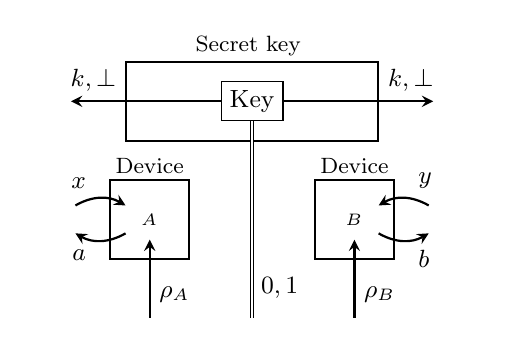
\begin{tikzpicture}[
sArrow/.style={->,>=stealth,thick},
thinResource/.style={draw,thick,minimum width=3.2cm,minimum height=1cm},
sqResource/.style={draw,thick,minimum width=1cm,minimum height=1cm},
pnode/.style={minimum width=.6cm,minimum height=.5cm}]

\small

\def\t{2.3} %1.6+.7
\def\u{.25}
\def\v{.75}
\def\w{1.3} 
\def\z{2}

\node[thinResource] (keyBox) at (0,\v) {};
\node[yshift=-1.5,above] at (keyBox.north) {\footnotesize
  Secret key $\aK$};

\node[draw] (key) at (0,\v) {Key};
\node (a1) at (-\t,\v) {};
\node (b1) at (\t,\v) {};
\node (eve) at (0,-\z) {};

\draw[sArrow] (key) to node[pos=.85,auto] {$k,\bot$} (b1.center);
\draw[sArrow] (key) to node[pos=.85,auto,swap] {$k,\bot$} (a1.center);
\draw[double] (eve.center) to node[pos=.15,auto,swap] {$0,1$} (key);


\node[pnode] (a2) at (-\t-\u,-\v) {};
\node[pnode] (b2) at (\t+\u,-\v) {};

\node[sqResource] (da) at (-\w,-\v) {$\aD_A$};
\node[yshift=-1.5,above] at (da.north) {\footnotesize
  Device};
\node[pnode] (dan) at (-\w,-\v) {};
\node[sqResource] (db) at (\w,-\v) {$\aD_B$};
\node[yshift=-1.5,above] at (db.north) {\footnotesize
  Device};
\node[pnode] (dbn) at (\w,-\v) {};

\node (eveq1) at (-\w,-\z) {};
\node (eveq2) at (\w,-\z) {};

\draw[sArrow] (eveq1.center) to node[pos=.3,auto,swap] {$\rho_A$} (dan);
\draw[sArrow] (eveq2.center) to node[pos=.3,auto,swap] {$\rho_B$} (dbn);

\draw[sArrow,bend left] (a2) to node[pos=.4,auto] {$x$} (dan);
\draw[sArrow,bend left] (dan) to node[pos=.6,auto] {$a$} (a2);
\draw[sArrow,bend right] (b2) to node[pos=.4,auto,swap] {$y$} (dbn);
\draw[sArrow,bend right] (dbn) to node[pos=.6,auto,swap] {$b$} (b2);

\end{tikzpicture}


\caption[Reusing devices]{\label{fig:open.di}An ideal world in which a
  secret key is produced by $\aK$ and new devices $\aD_A$ and $\aD_B$
  independent from $\aK$ are accessible to the players..}
\end{figure}

Unfortunately, no DI-QKD protocol has ever been shown to construct the
ideal system from \figref{fig:open.di} and it might well be impossible
to do so. But even if this is the case, it does not exclude that one
can construct an ideal system that is stronger than just the shared
secret key considered in \secref{sec:alternative.di}, e.g., one in
which the devices have some partial independence from the key or are
fully independent in certain contexts.\footnote{Context restricted
  composability is a promising research path for protocols that do not
  construct the desired ideal resource. Its investigation has been
  initiated in \textcite{JM18}, and is beyond the scope of this
  review.}

We note that weaker models such as measurement\-/device\-/independent
(MDI) QKD \--- see \secref{sec:alternative.semi} \--- do not
suffer from the same problem of device reuse as DI-QKD. The reason is
that in MDI-QKD one does not need to make any assumption about the
measurement devices at all (the adversary does the measurements for
the honest players), whereas in DI-QKD one has to assume that no
unauthorized information leaves the devices.

% This may be seen as a lack of composability: if one runs
% the protocol once in an isolated environment, the outcome remains
% secret, but if we consider a larger context where the device may be
% reused, some vital information may leak to the adversary.

% The security definitions used in device independent cryptography are
% inspired by their device dependent counterparts, e.g., the trace
% distance criterion. But unlike for the trace distance criterion, it
% has so far not been shown that these equations can be derived from a
% composable framework. In fact, it is not clear exactly what resources
% are constructed by these protocols. It is therefore an important open
% problem to develop such a framework, which enables a proper security
% analysis of device independent protocols.


\subsection{Computational security}
\label{sec:open.computational}

Computational security is a fairly unexplored area of quantum
cryptography. The main motivation for studying this is to achieve
results that are not possible with information\-/theoretic
security. For example, in \secref{sec:dqc} we mentioned a
computationally secure protocol for delegated quantum computation with
a classical client \cite{GV19}, which is believed not to be possible
with information\-/theoretic security~\cite{ACGK19}. The
computationally secure message transmission from
\secref{sec:computational} allows keys to be reused without the extra
communication required by QKD (\secref{sec:qkd}) or key recycling
(\secref{sec:recycle}) \--- and thus, without the possibility of an
adversary interrupting this communication and preventing the key from
being reused. And the work from \textcite{Unr13} discussed in
\secref{sec:mpc.ever} removes the need for a shared secret key in QKD
by using signature cards instead.

One may essentially analyze any area of cryptography with
computational security to study how assumptions needed for
information\-/theoretic security may be weakened in the computational
setting. There is however no single way to model computational
assumptions, and important open questions in the field are to identify
the (best) ways of doing this. Most frequently, one proves a
reduction, i.e., if some distinguisher can guess whether it is
interacting with the real or ideal system, then this distinguisher can
be used to solve some problem which is believed to be hard. In
\secref{sec:computational} we reviewed the finite reductions from
\textcite{BMPZ19}, in which the probability of a distinguisher $\fD$
distinguishing the real and ideal worlds is bounded by the probability
of this distinguisher being successfully used \--- as part of a new
distinguisher $\fD'$ \--- to distinguish a pseudo\-/random function
from a uniform random function; see also \textcite{Rog06} for a
discussion of reductions.

Another way to define computational security would be to define an
ideal resource that falls under the control of the adversary if she
can solve some problem believed to be hard (e.g., find a collision for
a hash function). This is essentially the ``identical-until-bad''
concept of \textcite{BR06}, but adapted to composable security instead of
game-based security. To the best of our knowledge, this paradigm remains
completely unexplored in quantum cryptography.

Other works such as \textcite{CCLVW17} bound adversaries by
circuit sizes. It is not clear how to model that in a finite,
composable framework, and is important open work.



\subsection{Other setup assumptions}
\label{sec:open.other}

When a security definition is considered ``not composable'', it often
has some (setup) assumption hard-coded in it, which is not present in
the obvious composable definition, and is therefore strictly
weaker. By modeling this assumption in a composable framework, one can
get another, equivalent composable definition. We illustrated this
in \secref{sec:alternative.memoryless} by explaining how a definition for QKD based on the accessible information, which is normally not composable, can be turned into a composable
one within a model where an adversary has no (long term) quantum
memory.

Similar techniques have been used by \textcite{Unr11} to obtain
commitments in the bounded storage model. While it follows from
\textcite{VPdR19} that coin flipping and bit commitment are impossible
in a bounded storage model without further assumptions,
\textcite{Unr11} avoids these by putting a bound on the number of
times a protocol can be run in parallel, and designing protocols that
are secure for this limited number of compositions.\footnote{This
  effectively restricts what the distinguisher/environment may do to
  distinguish the real and ideal systems, since the bound on the
  number of executions of a protocol applies to the distinguisher as
  well.} Likewise, \textcite{Pro20} has made extra setup assumptions
in the relativistic model to avoid the impossibility results of
\textcite{VPdR19}.
  
  There are numerous works where security is proved based on the assumption that adversaries are restricted. For example, adversaries cannot share entanglement in
\textcite{BCFGGOS14}, the adversaries' memory size is bounded in
\textcite{DFSS07,DFSS08}, the adversaries' memory is noisy in
\textcite{WST08,STW09,KWW12}, or adversaries can only perform local
operations on single qubits and communicate classically in
\textcite{Liu14,Liu15}. It remains open how to model these assumptions
to get composable security statements and prove in what setting such
protocols are secure. Similarly, to capture position\-/based
cryptography \textcite{Unr14} uses a model of circuits with positions in
space\-/time. Here too, it is not clear how to fit these results in a
composable framework and identify the resource that is constructed by these
protocols.


%%% Local Variables:
%%% TeX-master: "main.tex"
%%% End:









\bibliographystyle{alpha}
\bibliography{refs}
\appendix
\section{Free Probability Primer}
\label{sec:app}

There are many excellent books on free probability theory. In particular, we refer to the book \cite{NS06} for more details than the brief introduction given here.

\subsection{Preliminaries}
\label{sec:free}



\paragraph{$C^*$-algebras.} Let $\CA$ be a unital $C^*$-algebra. For our purposes, we can think of this as an algebra of bounded operators on a complex Hilbert space which is self-adjoint ($a \in \CA$
 implies $a^* \in \CA$), closed in the operator norm $\|\cdot\|$, and contains the identity ($\bone \in \CA$). A faithful trace $\phi$ on $\CA$ is a continuous linear functional $\phi: \CA \to \C$ that is  unital ($\phi(\bone)=1$), positive $\phi(aa^*) \ge 0$, and $\phi(aa^*) = 0$ iff $a=0$. 
 
 The pair $(\CA, \phi)$ where $\CA$ is a unital $C^*$-algebra and $\phi$ is a faithful trace on $\CA$ is called a $C^*$-\emph{probability space}. Elements of $\CA$ are called non-commutative random variables. An example of a $C^*$-probability space is the class $(M_n(\C), \tr_n)$, which is the class of $n \times n$ complex matrices with the normalized trace  functional defined as $\tr_n(M) = \frac{1}{n} \sum_{i=1}^n {M_{ii}}$. General $C^*$-probability spaces allow us to extend these definitions to infinite-dimensional operators, which are needed to define a non-commutative analog of independence called \emph{free independence}. Faithfulness of the trace $\phi$ then ensures that $\|a\|= \lim_{m \to \infty} \phi((aa^*)^m)^{1/2m}$ (see \cite[Proposition 3.17]{NS06}). In particular, this allows one to compute the norm $\|\cdot\|$ by using the trace method and taking higher powers of the trace functional $\phi$, as we will see below.


\paragraph{Free Independence.} Let $(\CA, \phi)$ be a $C^*$-probability space and let $\{\CA_i\}_{i=1}^n$ be unital $*$-subalgebras of  $\CA$. They are said to be \emph{free} (or \emph{freely independent}) if for all $k \in [n]$, for all indices $i_1, \ldots, i_k \in [n]$, and for all $a_1 \in \CA_{i_1}, \ldots, a_k \in \CA_{i_k}$ satisfying $\phi(a_1)=\ldots =\phi(a_k)=0$, the joint \emph{free moment},
\[ \phi(a_1 \cdots a_k) = 0\]
whenever $j_1 \neq j_2, j_2\neq j_3, \ldots, j_{k-1} \neq j_k$, that is, the free moments vanish when all the neighboring elements in the sequence $a_1, \ldots, a_k$ come from  subalgebras with distinct indices, for example, $\phi(a_1a_2a^*_1a^*_2a_3a_2)=0$.

{Non-commutative random variables $a_1, \ldots, a_n \in (\CA, \phi)$ are said to be free if the subalgebras $\{\CA_i\}_{i=1}^n$ are free, where $\CA_i$ is the unital $*$-subalgebra  generated by $a_i$ (the linear span of all monomials $a^{\eps_1}_ia^{\eps_2}_i\cdots a^{\eps_r}_i$ where $\eps_1, \ldots, \eps_r \in \{1,*\}$ and $r \in \N \cup \{0\}$). Note that the corresponding unital $C^*$-subalgebras obtained by taking the norm closure of each $\CA_i$ are also freely independent in this case (see \cite[Exercise 5.23]{NS06}).}



We remark that the set of free non-commutative random variables is an empty set if the underlying $C^*$-probability space is finite (for instance $(M_n(\C), \tr_n)$), so to find non-trivial examples one needs to work with infinite-dimensional $C^*$-probability spaces. 

\paragraph{Free Haar Unitaries and Free Groups.} Let $(\CA, \phi)$ be a $C^*$-probability space. An element $u \in \CA$ is a \emph{Haar unitary} if it is a unitary, i.e.\ $uu^*=u^*u= \bone$, and if $\phi(u^k) = 0$ for all non-zero integers $k$. A family $S = \{u_1, \ldots, u_n\} \in \CA$ in a $C^*$-probability space $(\CA, \phi)$ is called a \emph{free Haar unitary family} if each $u \in S$ is a Haar unitary and if $u_1, \ldots, u_n$ are free. For notational convenience, let us define $S^* = \{u^*_1, \ldots, u^*_n\}$ to be the set of corresponding adjoints.

One can give a very precise condition when the trace $\phi$ evaluated on a non-commutative monomial in the $u_i$'s vanishes in terms of the free group. The \emph{free group} $F_n$ with generating set $S$ is an infinite discrete group constructed as follows: a word is defined to be product of elements of $S \cup S^*$ with $\bot$ denoting the empty word that contains no symbols. A word is called reduced if it does not contain a sub-word of the form $g g^{*}$ or $g^{*} g$ for $g \in S$. Given a word that is not reduced, the process of repeatedly removing such sub-words until it becomes reduced is called reduction. The free group $F_n$ consists of all reduced words that can be built from the symbols in $S \cup S^*$ with the group operation being a product of words followed by reduction. The identity is the empty word $\bot$. 

For a $d$-tuple $\bi  = (i_1, \ldots, i_d) \in [m]^d$, let $u_{\bi}$ denote the non-commutative monomial $u_{i_1}\cdots u_{i_d}$ and write $u^*_{\bi} = (u_{\bi})^* = u^*_{i_d} \cdots u^*_{i_1}$. Let $\bi_1,\ldots, \bi_t, \bj_1, \ldots, \bj_t$ each be a $d$-tuple in $[m]^d$ and consider the degree-$2td$ non-commutative monomial $w = u^{}_{\bi_1}u^*_{\bj_1} u^{}_{\bi_2}u^*_{\bj_2}\cdots u^{}_{\bi_t}u^*_{\bj_t}$. Note that a degree-$2td$ monomial $w$ corresponds to an ordered $2td$-tuple of variables. To illustrate, if $t=1, m=3$ and $\bi_1=(1,2,3)$ and $\bj_1 = (2,2,1)$, then $w = u_{1}u_2u_3(u_2u_2u_1)^* = u_{1}u_2u_3u_1^*u^*_2u^*_2$ and corresponds to the ordered tuple $(u_1, u_2, u_3, u^*_1, u^*_2, u_2^*)$. We can also interpret $w$ as a word in the free group by applying the reduction rules. Then the next proposition follows from the definitions of free independence and Haar unitaries.

\begin{proposition} \label{prop:word}
    $\phi(w) = 1$ iff $w$ reduces to identity in the free group $F_n$, and $\phi(w) = 0$ otherwise.
\end{proposition}

 For a monomial $w$ that reduces to identity in the free group, the procedure for reducing a monomial $w$ as above first removes some adjacent pair $u_k$ (at index $i$) and $u^*_k$ (at index $j)$, then removes another adjacent pair $u_l$ and $u^*_l$ in the resulting word and so on and so forth until we reach the empty word. In particular, this reduction procedure produces a pairing of the set $[2td]$ where the index $i$ and $j$ are paired up iff the  variables at indices $i$ and $j$ in the monomial $w$ are $u_k$ and $u^*_k$ (for some $k$). Moreover, this pairing is what is called a \emph{non-crossing} pairing defined below (see \figref{fig:non-crossing}). Note that a monomial could be reduced to identity in different ways, so there could be many such non-crossing pairings for a given monomial $w$.



%\vspace{5mm}
\begin{figure}[h!]
    \centering
   \includegraphics[width=0.6\textwidth]{noncrossing.pdf}
   \caption{\footnotesize A non-crossing $*$-pairing resulting from the reduction of a word to identity in the free group}
    \label{fig:non-crossing}
\end{figure}

\paragraph{Non-crossing Pairings.}  For any even integer $n$, let $\CP_2(n)$ denote the set of all pairings of $n$, that is, the set of all partitions of $[n]$ where each block is of size two. Let $\NC_2(n) \subseteq \CP_2(n)$ denote the set of all  pairings of $[n]$ that are non-crossing,\emph{ i.e.} pairings  which do not contain blocks $\{i_1,i_3\}, \{i_2, i_4\}$ such that $i_1 < i_2 < i_3 < i_4$. 

For integers $d,m$, we divide the set $[2dm]$ into $2m$ consecutive blocks of $d$ elements each and color consecutive blocks alternatively with red and blue. Formally, for $i \in [2m]$, the elements $\{(i-1)d+1,\ldots, id\}$ are colored red if $i$ is odd and blue if $i$ is even. We define $\NC_2^*(d,m) \subseteq \NC_2(2dm)$ to be the set of those non-crossing pairings of $[2dm]$ which only pair up elements of different colors. We call any pairing in $\NC_2^*(d,m)$ a $*$-pairing.

We shall need the following combinatorial fact about the number of $*$-pairings (see \cite[Corollary 3.2]{KS05}).

\begin{lemma}\label{lem:catalan-fuss}
    For all $d, m$, the number of $*$-pairings  $|\NC_2^*(d,m)|$ equals the Fuss-Catalan number
    \[ 
    C_{d,m} = \frac{1}{m}\binom{m(d+1)}{m-1} = O\left(\frac{(d+1)^{m(d+1)}}{\left(d+\frac1m\right)^{md+1}}\right).
    \] 
\end{lemma}




\subsection{Proofs of \lref{thm:trace} and \thmref{thm:op-norm}}



\begin{proof}[Proof of \lref{thm:trace}]
    Writing $u^*_\bi = (u_\bi)^*$ for a tuple $\bi$ and using linearity of $\phi$, we have that 
    \[ 
    \phi[p(u_1, \ldots, u_t) (p(u_1, \ldots, u_t))^*] =  \sum_{|\bi|,|\bj| \le d} c_{\bi}c_{\bj} \phi(u_{\bi}u^*_{\bj}).
    \]
    From \pref{prop:word}, the term $\phi(u_{\bi}u^*_{\bj})$ is 1 iff $u_{\bi}u^*_{\bj}$ reduces to identity in the free group $F_t$ with generators $u_1, \ldots, u_t$. For the right-hand side above, this only happens when $\bi=\bj$ and thus these are the only non-zero terms. Thus, 
    \[ \phi[p(u_1, \ldots, u_t) (p(u_1, \ldots, u_t))^*] =  \sum_{|\bi| \le d} |c_{\bi}|^2. \qedhere\]
\end{proof}

Below we present the argument of Kemp and Speicher \cite{KS05}. Our exposition follows their proof closely but we adapt it to our context.
\begin{proof}[Proof of \thmref{thm:kemp-speicher}]
     We have that $\|p\| = \lim_{m \to \infty} \left(\phi((pp^*)^m)\right)^{1/(2m)}$ by the faithfulness of the trace $\phi$. Writing $u^*_\bj = (u_\bj)^*$ for a tuple $\bj$, we can compute 
    \begin{align*}
         \phi((pp^*)^m) = \sum_{\substack{|\bi_1|=\ldots=|\bi_m|=d\\|\bj_1|=\ldots=|\bj_m|=d}} c_{\bi_1}\cdots c_{\bi_m}c_{\bj_1}\cdots c_{\bj_m} \phi(u^{}_{\bi_1}u^*_{\bj_1} \cdots u^{}_{\bi_m}u^*_{\bj_m}).
    \end{align*}
    
    Since $u_1, \ldots, u_t$ are free Haar unitaries, \pref{prop:word} implies that $\phi(u^{}_{\bi_1}u^*_{\bj_1} \cdots u^{}_{\bi_m}u^*_{\bj_m})$ is 1 iff the word $u^{}_{\bi_1}u^*_{\bj_1}\cdots u^{}_{\bi_m}u^*_{\bj_m}$ reduces to identity in the free group $F_t$, and is 0 otherwise. Moreover, if the word corresponding to the index $(\bi_1,\bj_1, \ldots, \bi_m,\bj_m)$ reduces to identity, then there exists a $*$-pairing $\pi \in \NC_2^*(d,m)$ which matches only variables with the same indices. We call any such $*$-pairing $\pi$ consistent with the $2dm$-tuple $(\bi_1,\bj_1, \ldots, \bi_m,\bj_m)$ and denote this by the indicator function $\ind[\pi, \bi_1,\bj_1, \ldots, \bi_m,\bj_m]$.
    
    The above implies that we may bound 
    \[ \phi(u^{}_{\bi_1}u^*_{\bj_1} \cdots u^{}_{\bi_m}u^*_{\bj_m})  \le \sum_{\pi \in \NC^*_2(d,m)} \ind[\pi, \bi_1,\bj_1, \ldots, \bi_m,\bj_m],\]
    where the inequality occurs because there could be multiple $*$-pairings consistent with a tuple. We thus have that 
    \begin{align*}
         \phi((pp^*)^m) &\le \sum_{\substack{|\bi_1|=\ldots=|\bi_m|=d\\|\bj_1|=\ldots=|\bj_m|=d}} c_{\bi_1}\cdots c_{\bi_m}c_{\bj_1}\cdots c_{\bj_m} \sum_{\pi \in \NC^*_2(d,m)} \ind[\pi, \bi_1,\bj_1, \cdots, \bi_m,\bj_m]\\
         &= \sum_{\pi \in \NC^*_2(d,m)}  \sum_{\substack{|\bi_1|=\ldots=|\bi_m|=d\\|\bj_1|=\ldots=|\bj_m|=d}} c_{\bi_1}\cdots c_{\bi_m}c_{\bj_1}\cdots c_{\bj_m} \ind[\pi, \bi_1,\bj_1, \cdots, \bi_m,\bj_m].
    \end{align*}
    
    If a term corresponding to a fixed $*$-pairing $\pi$ is non-zero, then the list of indices $(\bi_1, \ldots, \bi_m)$ is the same as $(\bj_1, \ldots, \bj_m)$ up to the exact ordering. Let us relabel $(\bi_1, \ldots, \bi_m) = (a_1, \ldots, a_{dm})$ and $(\bj_1, \ldots, \bj_m) = (b_1, \ldots, b_{dm})$ and let $c_{a_1, \ldots, a_{dm}} = c_{\bi_1}\ldots c_{\bi_m}$ and $c_{b_1, \ldots, b_{dm}} = c_{\bj_1}\cdots c_{\bj_m}$. Since $\pi$ gives a non-crossing bijection between the two lists $(a_1, \ldots, a_{dm})$ and $(b_1,\ldots, b_{dm})$, it holds that $c_{b_1, \ldots, b_{dm}} = c_{\pi(a_1),\ldots, \pi(a_{dm})}$. Thus, the above sum is
    \begin{align*}
        \ \phi((pp^*)^m) &\le \sum_{\pi \in \NC^*_2(d,m)}  \sum_{a_1, \ldots, a_{dm}} c_{a_1, \ldots, a_{dm}} c_{\pi(a_1),\ldots, \pi(a_{dm})}\\
        \ &\le \sum_{\pi \in \NC^*_2(d,m)} \left(\sum_{a_1, \ldots, a_{dm}} |c_{a_1, \ldots, a_{dm}}|^2\right)^{1/2}
        \left(\sum_{a_1,\ldots, a_{dm}} |c_{\pi(a_1),\ldots, \pi(a_{dm})}|^2\right)^{1/2},
    \end{align*}    
     where the inequality follows from Cauchy-Schwarz. The two internal summations are exactly the same since the summation is over all $dm$ tuples of indices and $\pi$ is a bijection. Switching back to the old indexing scheme, the internal summation then equals 
     \[  \sum_{a_1, \ldots, a_{dm}} |c_{a_1, \ldots, a_{dm}}|^2 = \sum_{\substack{|\bi_1|=\ldots=|\bi_m|=d}} |c_{\bi_1}\cdots c_{\bi_m}|^2 = \left(\sum_{|\bi|=d} |c_{\bi}|^2\right)^m.\] 
    Overall, we have
     \begin{align*}   
        \  \phi((pp^*)^m) &\le |\NC^*_2(d,m)|\left(\sum_{|\bi|=d} |c_{\bi}|^2\right)^m.
    \end{align*}
    Using \lref{lem:catalan-fuss} to bound the number of $*$-pairings,
    \[ |\NC^*_2(d,m)| = C_{d,m} = \frac{1}{m}\binom{m(d+1)}{m-1} = O\left(\frac{(d+1)^{m(d+1)}}{\left(d+\frac1m\right)^{md+1}}\right).\]
    Thus, taking the $m$-th root in the limit $m \to \infty$ yields
    \[ \|p\|^2 = \lim_{m \to \infty}  \phi((pp^*)^m)^{1/m} = \frac{(d+1)^{d+1}}{d^d}\left(\sum_{|\bi|=d} |c_{\bi}|^2\right) \le e(d+1) \left(\sum_{|\bi|=d} |c_{\bi}|^2\right).\]
    This completes the proof of the theorem.
\end{proof}






\end{document}
